\chapter{Context (Estat de l'art)}\label{C:compaginacio}

\section{Ús lliure de RF}
Amb l'establiment de les bandes ISM (Afegir referencia) es crea la possibilitat per el públic general utilitzar comunicació inal·làmbrica amb molta facilitat. Això es deu a que l'establiment de les bandes ISM està acceptat de manera (mes o menys(?)) de la mateixa manera internacionalment.
Això facilita el disseny de productes per al consumidor habitual que ràpidament veu els avantatges de la comunicació inal·làmbrica entre dispositius.
En aquest entorn sorgeix la necessitat d'establir estandards entre le companyies principals dels sectors. Per definir els estandards s'agrupen les companyies i formen grups com al WIFI Alliance o ...

\subsection{Wifi}
La tecnologia de comunicació més popular avui en dia és la WIFI, dissenyada originalment als anys (?) i establerta als anys (?) orientada a permetre una connexió (* bona) i sense consideració per les interferències entre si mateixa que no es podien preveure llavors.  
- Avantatges
- Innovació
- Evolució

\subsection{Bluetooth Classic}
Bluetooth enlloc de estar orientat a donar connexió a internet estava orientat a connectar dispositius entre si (punt a punt) per a la transferència de fitxers com contactes o fotografies.
Posteriorment es va poder aconseguir velocitats suficients pel \textit{streaming} de música en temps real.
Junt amb l'arribada dels telèfons intel·ligents els auriculars inal·làmbrics es van fer populars i també es va establir la dominància de bluetooth per a escoltar música sense cables.
Amb aquest objectiu es va millorar bluetooth per tal de ser més resistent a interferències i a poder transmetre més velocitat per poder transmetre música d'alta fidelitat.
Per un altre costat però va començar a sorgir el Internet of Things, basat en tenir molts dispositius connectats i això va generar necessitats que no es podien cobrir amb les tecnologies desenvolupades anteriorment.

\section{MANETS}
Bluetooth classic no permetia ni tenir més d'una connexió establerta amb dispositius i l'arquitectura feia que s'utilitzés bastanta energia per establir i mantenir una connexió encara que es volguessin transmetre molt poques dades.
Aquestes limitacions feien que fos necessari definir nous protocols que estiguessin orientats a connexions de poques dades cap a més d'un dispositiu i que utilitzessin el mínim de energia possible.

\subsection{BLE}
Bluetooth Low Energy no té cap relació amb Bluetooth Classic pel que fa a l'arquitectura del protocol. Tot i compartir nom (perque?) queda clar que no estem parlant del mateix amb el simple fet que no son compatibles entre sí. Tot i així comparteixen l'ús de la banda freqüencial de 2,4 GHz igual que altres protocols sense fils. Al 2016 es va anunciar la versió 5.0 anomenada Bluetooth 5 (sense el punt)[cita] i se li va canviar el nom (aclariment).

% Diferencies entre classic i low energy

\subsection{Altres Protocols}
Bluetooth Low Energy no és l'únic protocol orientat a la connexió de dispositius amb baix consum energètic. També existeixen els següents protocols:
Zigbee, utilitzat en Philips Hue
Zwave Ring (home security)
6lowpan
insteon
lorawan

% Prodcutes que utilitzen cadascun

\subsection{Comparació}
Tot i que els protocols tenen molt en comú cada un es diferencia de la resta en els detalls, a continuació veiem una comparació de les capacitats de cada un dels protocols

\section{BLE Stack}
Un cop vistes les característiques generals del protocol cal entendre com funciona per dins.
En entrar en detall queda clar com el protocol s'ha dissenyat de forma molt flexible 

\begin{figure}[h]
	\begin{center}
		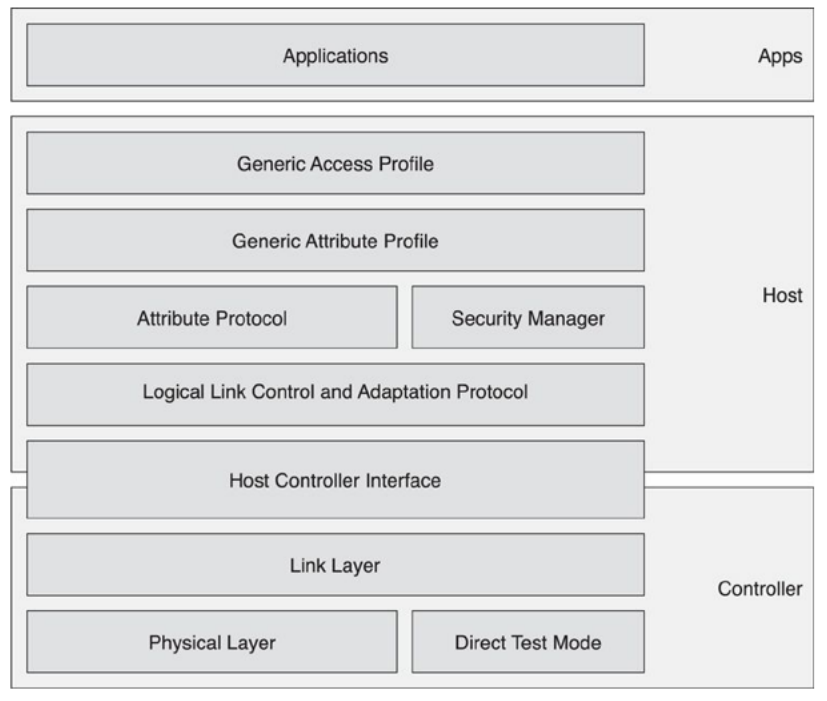
\includegraphics[width=0.8\textwidth]{./images/BLE_Stack.png}
		\caption{Pila de BLE \cite{ble_stack}}
		\label{ble_stack}
	\end{center}
\end{figure}


\subsection{Controller}
\subsubsection{PHY}
La capa física és la que s'encarrega de la communicació anal·lògica modulant i desmodulant les senyals.
Tal i com ja s'ha comentat abans treballa a la banda de 2.4 GHz en 40 canals diferents

\subsubsection{Link Layer}
\subsection{Host}
\subsubsection{L2 Cap}
\subsubsection{SMP}
\subsubsection{ATT}
\subsubsection{GATT}
\subsubsection{GAP}
\subsection{Application}

